\section{Interference Differential Cross Sections}
In Figure \ref{fig:sig_i}, the interference differential cross section for energetic deuterons colliding with tritons is shown for various incident energies. Looking at Figure \ref{fig:sig_i}, as $\mucm \rightarrow 1$ the interference differential cross section oscillates between positive and negative values of increasing magnitude. Negative differential cross sections have no physical meaning, and therefore the interference differential cross section must be combined some other differential cross section such that the resulting differential cross section is always positive.

\begin{figure}[!htb]
    \centering
    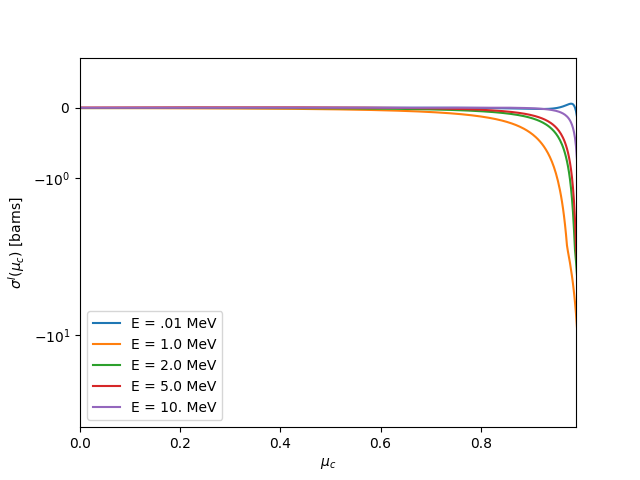
\includegraphics[scale=0.75]{../figures/proposed_work/sig_i_dt.png}
    \caption{Interference scattering differential cross section for deuterons colliding with tritons at 1.0 MeV}
    \label{fig:sig_i}
\end{figure}